\documentclass[a4paper]{article}
\usepackage[english]{babel}
%
% English translation of the original Spanish manuscript.
% Equations and notation were preserved where possible; a few physics/LaTeX issues
% were corrected and are listed separately in the accompanying notes.
%
\usepackage{amsmath}
\usepackage{amsfonts}
\usepackage{amssymb}
\usepackage{bbold}
\usepackage{graphicx}
\usepackage{blindtext}
\usepackage{hyperref}

\begin{document}
\pagenumbering{arabic}

\Large
 \begin{center}
Introduction to Quantum Circuits and\\
Quantum Teleportation

\hspace{10pt}

% Author names and affiliations
\large
%Lic. Julio A. Medina$^1$ \\
Julio A. Medina$^1$ \\
\hspace{10pt}
\small
$^1$ Universidad de San Carlos\\
School of Physical and Mathematical Sciences\\
Master's Program in Physics\\
\href{mailto:julioantonio.medina@gmail.com}{julioantonio.medina@gmail.com}\\

\end{center}

\hspace{10pt}

\normalsize
\section{The Origins of Quantum Computing}
Quantum computing was born from Richard P. Feynman's desire to analyze and simulate quantum systems by means of computational systems. This quickly led to the realization that the problem grows exponentially with respect to the number of particles to be simulated, which means that the computational cost grows in the same way. This made the simulation of such quantum systems extremely difficult. In 1981, Feynman\cite{Feynman} published a seminal article that planted the seed for the creation of quantum computing systems capable of simulating systems of quantum nature more effectively. \\

\section{From Bits to Qubits}
In classical computing, states or bits are either $1$ or $0$. In quantum mechanics, however, due to the principle of superposition of states, a qubit can be found in a superposition of states; that is, it can be simultaneously in $1$ and $0$. These superpositions allow computations to be performed over several states simultaneously; in other words, computational processes are naturally parallelized. This makes it possible to create quantum algorithms with exponential improvements in computational performance. However, due to the collapse of the wave function, when a measurement is performed on a superposition state, the state collapses into one of the eigenstates of the operator used to perform the measurement. \\
For this reason, quantum algorithms are designed in such a way that the correct answer is amplified; that is, the correct answer resonates in the wave function. This makes the design of quantum algorithms a nontrivial task.

\subsection{Dirac Notation}
Dirac notation is used to describe quantum states. Quantum states are vectors in Hilbert space. They may be finite-dimensional vectors, or they may describe continuous quantities and therefore be infinite-dimensional vectors. The English physicist Paul Dirac popularized what is now called Dirac notation in order to make calculations in quantum mechanics more compact.

The ket is defined as
\begin{equation}
|a\rangle=
	\begin{pmatrix}
		a_1\\
		a_2
	\end{pmatrix}
\end{equation}
where $a_1, a_2 \in \mathbb{C}$. The bra is defined as the row vector, or the vector in the dual space of the ket, as
\begin{equation}
\langle a|=
	\begin{pmatrix}
		a_1^*&a_2^*
	\end{pmatrix}
\end{equation}
where $a_1^*, a_2^* \in \mathbb{C}$ are the complex conjugates of $a_1, a_2$.

Bras and kets are related as follows:
\begin{equation}
\langle a|=|a\rangle^\dagger
\end{equation}
which is equivalent to
\begin{equation}
\begin{pmatrix}
		a_1\\
		a_2
	\end{pmatrix}^\dagger=
	\begin{pmatrix}
		a_1^*&a_2^*
	\end{pmatrix}.
\end{equation}
If $a_1=x+iy$, then $a_1^*=x-iy$ is its complex conjugate. The operator $\dagger$ gives the conjugate transpose of a vector or matrix.\\

The bracket is defined as the inner product, or scalar product, in Hilbert space:
\begin{equation}
\langle b | a\rangle=a_1b_1^*+a_2b_2^*=\langle a | b\rangle^*\in \mathbb{C}.
\end{equation}
The ket-bra, or outer product, is defined as
\begin{equation}
|a\rangle\langle b|=
	\begin{pmatrix}
		a_1 b_1^*& a_1 b_2^*\\
		a_2 b_1^*& a_2 b_2^*\\
	\end{pmatrix}.
\end{equation}

\subsection{Qubit Representation}
The representation of a qubit is naturally given by the spinors used to describe the Stern--Gerlach experiment, in which the spin of silver atoms is measured. These spinors are defined as
\begin{equation}\label{eq::qubit0}
|0\rangle\equiv
\begin{pmatrix}
		1\\
		0
	\end{pmatrix}
\end{equation}
as the quantum analogue of the state $0$ for a classical bit. For the classical state $1$, one uses
\begin{equation}\label{eq::qubit1}
|1\rangle\equiv
\begin{pmatrix}
		0\\
		1
	\end{pmatrix}.
\end{equation}
These quantum states are evidently orthonormal: $\langle 0 | 1\rangle=0$ and $\langle 0 | 0\rangle=\langle 1 | 1\rangle=1$. These two states form a basis. All quantum states are normalized,
\begin{equation}
\langle \psi | \psi\rangle=1,
\end{equation}
for example $|\psi\rangle=\frac{1}{\sqrt{2}}(|0\rangle+|1\rangle)$.

\section{Measurements}
Orthonormal bases are generally used to describe and measure quantum states, and that convention is followed here. During a measurement in the basis $\{|0\rangle, |1\rangle\}$, the state collapses either to $|0\rangle$ or to $|1\rangle$. These are the eigenstates of $\sigma_z$, the Pauli-$z$ matrix; see Section~\ref{sec::PauliMatrix}. This is known as a measurement in the $z$ basis.\\
There are infinitely many different bases in which measurements can be performed, but other common bases are $\{|+\rangle, |-\rangle \}$, defined as
\begin{equation}
|+\rangle\equiv\frac{1}{\sqrt{2}}(|0\rangle+|1\rangle),
\end{equation}
\begin{equation}
|-\rangle\equiv\frac{1}{\sqrt{2}}(|0\rangle-|1\rangle),
\end{equation}
which are the eigenvectors of the Pauli-$x$ matrix $\sigma_x$. As expected, another commonly used basis consists of the eigenvectors of the Pauli-$y$ matrix $\sigma_y$:
\begin{equation}
|+i\rangle\equiv\frac{1}{\sqrt{2}}(|0\rangle+i|1\rangle),
\end{equation}
\begin{equation}
|-i\rangle\equiv\frac{1}{\sqrt{2}}(|0\rangle-i|1\rangle).
\end{equation}

\subsection{Born's Rule}
The probability that the state $|\psi\rangle$ collapses during a projective measurement in the basis $\{|x\rangle, |x^\perp \rangle \}$ to the state $|x\rangle$ is given by
\begin{equation}
P(x)=|\langle x|\psi\rangle|^2.
\end{equation}
From the fact that normalized states are being used, one obtains, as expected,
\begin{equation}
\sum_i P(x_i)=1.
\end{equation}
Some examples are presented to illustrate this rule.\\

\noindent a. The state $|\psi\rangle=\frac{1}{\sqrt{3}}(|0\rangle +\sqrt{2}|1\rangle)$ is measured in the basis $\{|0\rangle, |1\rangle \}$. Calculate the corresponding probabilities:
\begin{equation*}
P(0)=\bigg |\langle 0|\frac{1}{\sqrt{3}}(|0\rangle +\sqrt{2}|1\rangle)\bigg |^2=\bigg|\frac{1}{\sqrt{3}}\langle 0|0\rangle+\sqrt{\frac{2}{3}}\langle 0|1\rangle \bigg |^2,
\end{equation*}
\begin{equation*}
P(0)=\bigg|\frac{1}{\sqrt{3}} \bigg|^2=\frac{1}{3},
\end{equation*}
\begin{equation*}
P(1)=\bigg|\sqrt{\frac{2}{3}} \bigg|^2=\frac{2}{3},
\end{equation*}
\begin{equation*}
P(0)+P(1)=1.
\end{equation*}

\noindent b. The state $|\psi\rangle=\frac{1}{\sqrt{2}}(|0\rangle-|1\rangle)$ is measured in the basis $\{|+\rangle, |-\rangle\}$. Find the corresponding probabilities:
\begin{equation*}
P(+)=\bigg| \langle +|\psi\rangle\bigg|^2=\bigg|\frac{1}{\sqrt{2}}(\langle 0| +\langle 1|)\cdot \frac{1}{\sqrt{2}}(|0\rangle -|1\rangle)\bigg|^2,
\end{equation*}
\begin{equation*}
P(+)=\frac{1}{4}\bigg|\langle 0|0\rangle-\langle 0|1\rangle+\langle 1|0\rangle-\langle 1|1\rangle\bigg|^2=0,
\end{equation*}
\begin{equation*}
P(-)=1.
\end{equation*}
This is expected because $\big| \langle -|\psi\rangle\big|^2=\big| \langle -|-\rangle\big|^2=1$ and $\big| \langle +|-\rangle\big|^2=0$, by the orthogonality property of these bases.

\section{Quantum Circuits}
The ``circuit model'' is used: a sequence of basic blocks that perform elementary computations. These basic blocks are known as gates.

\subsection{Single-Qubit Gates}
To make an analogy with classical logic gates, consider the classical NOT gate, represented in Figure~\ref{fig::NOT_gate}.
\begin{figure}[h]
\begin{center}
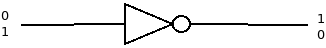
\includegraphics[scale=0.4]{./classicalNOT.png}
\end{center}
\caption{NOT gate}
\label{fig::NOT_gate}
\end{figure}
As can be seen in the figure, the operation performed by the NOT operator on a bit is trivial: it flips the bit state from $0$ to $1$ and vice versa.

One of the fundamental characteristics of quantum theory is that it is unitary. In other words, quantum operators---in this case quantum gates---must be unitary operators, that is, unitary matrices. For an operator $U$, this means that
\begin{equation}
U^\dagger U=\mathbb{1}.
\end{equation}
This implies that when a unitary operator acts on a ket, the magnitude of the ket does not change. Using Dirac notation, a unitary operator $U$ can be represented as a linear combination of ket-bras in the following way:
\begin{equation}
U=
	\begin{pmatrix}
		u_{00} &u_{01} \\
		u_{10} &u_{11}
	\end{pmatrix}=u_{00}|0\rangle\langle 0|+u_{01}|0\rangle\langle 1|+u_{10}|1\rangle\langle 0|+
	u_{11}|1\rangle\langle 1|.
\end{equation}

\subsubsection{Pauli Matrices}\label{sec::PauliMatrix}
The Pauli-$x$ matrix, $\sigma_x$, is defined as
\begin{equation}
\sigma_x=\begin{pmatrix}
		0 &1 \\
		1 &0
	\end{pmatrix}=|0\rangle\langle 1|+|1\rangle\langle 0|.
\end{equation}
This matrix serves as the quantum analogue of the NOT gate. To see this, it is enough to operate with the qubit representations defined in Equations~\ref{eq::qubit0} and \ref{eq::qubit1}:
\begin{equation}
\sigma_x|0\rangle=
	\begin{pmatrix}
		0 &1 \\
		1 &0
	\end{pmatrix}
	\begin{pmatrix}
		1 \\
		0
	\end{pmatrix}=
	\begin{pmatrix}
		0 \\
		1
	\end{pmatrix}=|1\rangle.
\end{equation}
Similarly, using Dirac notation, one obtains
\begin{equation}
\sigma_x|1\rangle=(|0\rangle\langle 1|+|1\rangle\langle 0|)|1\rangle=|0\rangle.
\end{equation}
This behavior is also known as a bit flip. The operator can also act on superpositions. The eigenvectors of $\sigma_x$ are the kets $|+\rangle$ and $|-\rangle$.\\

The Pauli-$z$ matrix, $\sigma_z$, is defined as
\begin{equation}
\sigma_z=
	\begin{pmatrix}
		1 &0 \\
		0 &-1
	\end{pmatrix}=|0\rangle\langle 0|-|1\rangle\langle 1|.
\end{equation}
The behavior of this matrix is described as a phase flip. To visualize this, let it act on the basis $\{|+\rangle, |-\rangle\}$:
\begin{equation}
\sigma_z|+\rangle=
	\begin{pmatrix}
		1 &0 \\
		0 &-1
	\end{pmatrix}\frac{1}{\sqrt{2}}
	\begin{pmatrix}
		1 \\
		1
	\end{pmatrix}=\frac{1}{\sqrt{2}}
	\begin{pmatrix}
		1 \\
		-1
	\end{pmatrix}=|-\rangle.
\end{equation}
In Dirac notation,
\begin{equation}
\sigma_z|-\rangle=(|0\rangle\langle 0|-|1\rangle\langle 1|)\frac{1}{\sqrt{2}}(|0\rangle-|1\rangle)=\frac{1}{\sqrt{2}}(|0\rangle+|1\rangle)=|+\rangle.
\end{equation}
The eigenvectors of the matrix $\sigma_z$ are the kets $|0\rangle$ and $|1\rangle$.\\

The Pauli-$y$ matrix, $\sigma_y$, is defined by
\begin{equation}
\sigma_y=
	\begin{pmatrix}
		0 &-i \\
		i & 0
	\end{pmatrix}=i|1\rangle\langle 0|-i|0\rangle\langle 1|.
\end{equation}
Note that $\sigma_y=-i \sigma_z\sigma_x=i\sigma_x\sigma_z$, so this gate can be interpreted, up to a global phase, as a sequence of a bit flip and a phase flip.\\
Any of the Pauli matrices $\sigma_x, \sigma_y, \sigma_z$ satisfies
\begin{equation}
\sigma_i^2=\mathbb{1}.
\end{equation}
The set formed by the Pauli matrices and the identity matrix is a basis for the space of $2\times2$ matrices.

\subsubsection{Hadamard Gate}
The Hadamard gate, $H$, is defined by
\begin{equation}
	H=
	\frac{1}{\sqrt{2}}
	\begin{pmatrix}
		1 & 1 \\
		1 &-1
	\end{pmatrix}=\frac{1}{\sqrt{2}}(|0\rangle\langle 0|+|0\rangle\langle 1|+|1\rangle\langle 0|-|1\rangle\langle 1|).
\end{equation}
The Hadamard gate is very useful because it creates superpositions of qubits. This is illustrated as follows:
\begin{equation}
H|0\rangle=\frac{1}{\sqrt{2}}(|0\rangle\langle 0|+|0\rangle\langle 1|+|1\rangle\langle 0|-|1\rangle\langle 1|)|0\rangle=\frac{1}{\sqrt{2}}(|0\rangle+|1\rangle),
\end{equation}
\begin{equation}
H|0\rangle=|+\rangle.
\end{equation}
Similarly,
\begin{equation}
H|1\rangle=|-\rangle.
\end{equation}
Since every quantum gate is unitary and $H$ is also a Hermitian operator, i.e. $H^\dagger=H$, one has
\begin{equation}
H|+\rangle=|0\rangle,
\end{equation}
\begin{equation}
H|-\rangle=|1\rangle.
\end{equation}
Therefore, the Hadamard gate can be used to change between the $x$ and $z$ bases.

\subsection{Multipartite Quantum States}
To describe multipartite quantum states, the tensor product is used. That is, if one has a state for a particle $|a\rangle$ and another state for a different particle $|b\rangle$, then the bipartite state is given by
\begin{equation}
|a\rangle \otimes |b\rangle=
	\begin{pmatrix}
		a_1 \\
		a_2
	\end{pmatrix}\otimes
	\begin{pmatrix}
		b_1 \\
		b_2
	\end{pmatrix}=
	\begin{pmatrix}
		a_1 b_1 \\
		a_1 b_2 \\
		a_2 b_1 \\
		a_2 b_2
	\end{pmatrix}.
\end{equation}
For example, suppose that system A is in the state $|1\rangle_A$ and system B is in the state $|0\rangle_B$. Then the total state of the composite system is given by
\begin{equation}
|10\rangle_{AB}\equiv |1\rangle_A\otimes |0\rangle_B=
	\begin{pmatrix}
		0 \\
		0\\
		1\\
		0
	\end{pmatrix}.
\end{equation}
An important observation about these states is that they are called uncorrelated. There are also bipartite states that cannot be written as $|\psi\rangle_A\otimes|\psi\rangle_B$. These are known as correlated states; for pure states, they are entangled states.\\

\subsection{Two-Qubit Gates}
To make an analogy with classical logic gates, consider the XOR logic gate, with truth table
\begin{center}
\begin{tabular}{ |c|c|c| }
 \hline
 $x$ & $y$ & $x\oplus y$ \\ \hline
 0   & 1   &   1\\
 1   & 0   &   1\\
 0   & 0   &   0\\
 1   & 1   &   0\\
 \hline
\end{tabular}
\end{center}
The XOR operator is not reversible. However, as discussed above, quantum theory is unitary and therefore reversible. To solve this issue, one uses the following two-qubit quantum gate, called CNOT, or controlled NOT, defined by
\begin{equation}
\text{CNOT}=
	\begin{pmatrix}
		1 & 0 & 0 & 0 \\
		0 & 1 & 0 & 0 \\
		0 & 0 & 0 & 1 \\
		0 & 0 & 1 & 0
	\end{pmatrix}=|00\rangle\langle 00|+|01\rangle\langle 01|+|10\rangle\langle 11|+|11\rangle\langle 10|.
\end{equation}
To see the effect of the CNOT gate, the following calculations are performed explicitly:
\begin{equation}
\text{CNOT}|00\rangle_{xy}=(|00\rangle\langle 00|+|01\rangle\langle 01|+|10\rangle\langle 11|+|11\rangle\langle 10|)|00\rangle,
\end{equation}
\begin{equation*}
\text{CNOT}|00\rangle=|00\rangle_{xy}.
\end{equation*}
Similarly,
\begin{equation}
\text{CNOT}|10\rangle_{xy}=(|00\rangle\langle 00|+|01\rangle\langle 01|+|10\rangle\langle 11|+|11\rangle\langle 10|)|10\rangle_{xy},
\end{equation}
\begin{equation*}
\text{CNOT}|10\rangle=|11\rangle_{xy},
\end{equation*}
\begin{equation}
\text{CNOT}|01\rangle_{xy}=(|00\rangle\langle 00|+|01\rangle\langle 01|+|10\rangle\langle 11|+|11\rangle\langle 10|)|01\rangle_{xy},
\end{equation}
\begin{equation*}
\text{CNOT}|01\rangle=|01\rangle_{xy},
\end{equation*}
\begin{equation}
\text{CNOT}|11\rangle_{xy}=(|00\rangle\langle 00|+|01\rangle\langle 01|+|10\rangle\langle 11|+|11\rangle\langle 10|)|11\rangle_{xy},
\end{equation}
\begin{equation*}
\text{CNOT}|11\rangle=|10\rangle_{xy}.
\end{equation*}

These results can be summarized in the following table, where the first two columns represent the input and the last two represent the output of the operation. In this case, with the control qubit being the qubit of system $x$, one obtains an analogue of the XOR gate, which is reversible as shown in the truth table.
\begin{center}
\begin{tabular}{ |c|c|c|c| }
 \hline
 $x$ & $y$ & $x$ & $x\oplus y$ \\ \hline
 0   & 1   &  0 &    1\\
 1   & 0   &  1 &    1\\
 0   & 0   &  0 &    0\\
 1   & 1   &  1 &    0\\
 \hline
\end{tabular}
\end{center}
A graphical representation of the CNOT gate, created with the Qiskit quantum computing API, can be seen in the following figure:
\begin{figure}[h]
\begin{center}
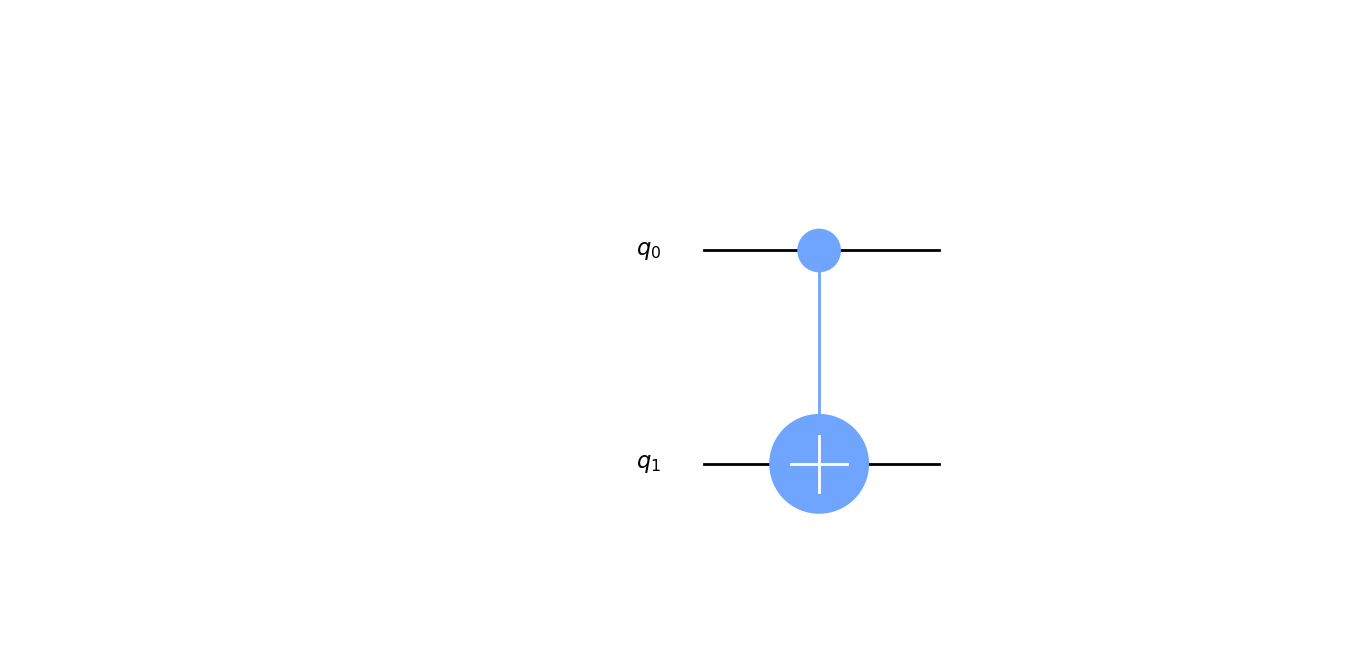
\includegraphics[scale=0.29]{./basic_CNOT_circuit.png}
\end{center}
\caption{CNOT quantum gate}
\label{fig::CNOT_gate}
\end{figure}\\
It is possible to show that quantum circuits can compute any classical Boolean-algebra function, the foundation of digital circuits and therefore of every classical computer.

\section{Quantum Entanglement}
If a pure state $|\psi\rangle_{AB}$ of systems A and B cannot be written as $|\phi\rangle_A\otimes |\gamma\rangle_B$, then the state $|\psi\rangle_{AB}$ is known as an entangled state. This is the definition of a correlated state; because only pure states are being considered here, every correlated state is also an entangled state.

\subsection{Bell States}
There are four states called Bell states, named after the physicist John Bell. Bell developed the so-called Bell inequalities\cite{Bell}, with which he addressed the Einstein--Podolsky--Rosen paradox. The Bell states are maximally entangled; that is, they maximally violate Bell inequalities. In addition, these Bell states form an orthonormal basis. They are defined as
\begin{equation}\label{eq::bell1}
|\psi^{00}\rangle\equiv \frac{1}{\sqrt{2}}(|00\rangle+|11\rangle),
\end{equation}
\begin{equation}\label{eq::bell2}
|\psi^{01}\rangle\equiv \frac{1}{\sqrt{2}}(|01\rangle+|10\rangle),
\end{equation}
\begin{equation}\label{eq::bell3}
|\psi^{10}\rangle\equiv \frac{1}{\sqrt{2}}(|00\rangle-|11\rangle),
\end{equation}
\begin{equation}\label{eq::bell4}
|\psi^{11}\rangle\equiv \frac{1}{\sqrt{2}}(|01\rangle-|10\rangle).
\end{equation}
In general, the Bell states can be written as
\begin{equation}
|\psi^{ij}\rangle\equiv \big( \mathbb{1}\otimes\sigma_x^j \sigma_z^i \big)|\psi^{00}\rangle.
\end{equation}
Correlation is not exclusive to quantum mechanics; it can also exist in classical systems. For example, suppose that a pair of gloves is distributed to two people without either person knowing the orientation of their glove (each glove is placed in a box whose interior cannot be seen). If the two people are then asked to travel by train in opposite directions and open the boxes half an hour later, the person who finds the right-handed glove will instantly know that the other person has the left-handed glove. However, quantum entanglement exhibits stronger correlations: if a pair of entangled particles is measured in a different basis, the correlation between the states is preserved. It is difficult to find a classical analogy for this situation. For instance, the Bell state can be written as
\begin{equation}
|\psi^{00}\rangle=\frac{1}{\sqrt{2}}\left(|++\rangle+|--\rangle\right),
\end{equation}
and a measurement can be performed in the basis $\{|++\rangle,|--\rangle\}$ while preserving the correlation.

\subsection{Creation of Bell States}
To create the Bell states, one can use a quantum circuit:
\begin{figure}[h]
\begin{center}
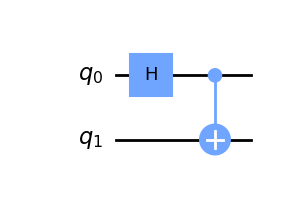
\includegraphics[scale=0.69]{./Bell_states_creation.png}
\end{center}
\caption{Quantum circuit for creating Bell states}
\label{fig::Bell_states_creation}
\end{figure}\\
This is equivalent to
\begin{equation}
\text{CNOT}\bigg((H_A\otimes\mathbb{1}_B)|ij\rangle_{AB} \bigg),
\end{equation}
with $i,j\in\{0,1\}$. To understand this circuit or calculation step by step, the following table shows the evolution of the initial state through the quantum circuit.
\begin{center}
\begin{tabular}{ |c|c|c| }
 \hline
 Initial State $|ij\rangle_{AB}$ & $(H_A\otimes\mathbb{1}_B)|ij\rangle_{AB}$ & Bell State \\ \hline
 $|00\rangle$  & $\frac{1}{\sqrt{2}}(|00\rangle+|10\rangle)$   &  $\frac{1}{\sqrt{2}}(|00\rangle+|11\rangle)$\\\hline
 $|01\rangle$  & $\frac{1}{\sqrt{2}}(|01\rangle+|11\rangle)$   &  $\frac{1}{\sqrt{2}}(|01\rangle+|10\rangle)$\\\hline
 $|10\rangle$  & $\frac{1}{\sqrt{2}}(|00\rangle-|10\rangle)$   &  $\frac{1}{\sqrt{2}}(|00\rangle-|11\rangle)$\\\hline
 $|11\rangle$  & $\frac{1}{\sqrt{2}}(|01\rangle-|11\rangle)$   &  $\frac{1}{\sqrt{2}}(|01\rangle-|10\rangle)$\\
 \hline
\end{tabular}
\end{center}

\subsection{Bell Measurement}
As mentioned several times, quantum circuits are reversible. Therefore, to go in the opposite direction of the Bell-state creation circuit presented above, one introduces a quantum circuit known as a Bell measurement, which reverses the process. The circuit is defined as
\begin{figure}[h]
\begin{center}
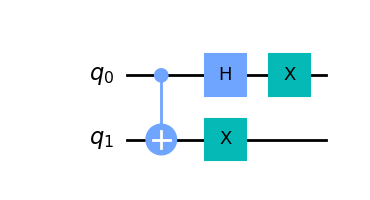
\includegraphics[scale=0.69]{./Bell_measurement.png}
\end{center}
\caption{Quantum circuit for Bell measurement}
\label{fig::Bell_measurement}
\end{figure}\\
This is equivalent to applying
\begin{equation}
(H\otimes\mathbb{1})\,\text{CNOT}\,|\psi^{ij}\rangle.
\end{equation}
This maps the Bell basis back to the computational basis, after which a standard computational-basis measurement can be performed.

\section{Quantum Teleportation}
The objective of the quantum teleportation protocol is the following: Alice wants to send a quantum state $|\phi\rangle_S$---unknown to Alice---to Bob,
\begin{equation}
|\phi\rangle_S=\alpha|0\rangle_S+\beta|1\rangle_S.
\end{equation}\\
However, Alice can only send two classical bits. Even if Alice knew the state, that is, the real values of $\alpha$ and $\beta$, two classical bits would not be enough to encode two real numbers. Nevertheless, by using the quantum properties of entanglement, Alice's objective can be achieved.

Suppose that Alice and Bob share a maximally entangled Bell state,
\begin{equation}
|\psi^{00}\rangle_{AB}=\frac{1}{\sqrt{2}}(|00\rangle_{AB}+|11\rangle_{AB}).
\end{equation}\\
Then the initial state of the system is
\begin{equation}
|\phi\rangle_S\otimes |\psi^{00}\rangle_{AB}=\frac{1}{\sqrt{2}}(\alpha|000\rangle_{SAB}+\alpha|011\rangle_{SAB}+\beta|100\rangle_{SAB}+\beta|111\rangle_{SAB}).
\end{equation}
This initial state can be rewritten as
\begin{equation}
\begin{split}
|\phi\rangle_S\otimes |\psi^{00}\rangle_{AB}=\frac{1}{2\sqrt{2}}\bigg[ &( |00\rangle_{SA}+|11\rangle_{SA})\otimes(\alpha|0\rangle_B+\beta|1\rangle_B)\\
&+(|01\rangle_{SA}+|10\rangle_{SA})\otimes(\alpha|1\rangle_B+\beta|0\rangle_B) \\
&+(|00\rangle_{SA}-|11\rangle_{SA})\otimes(\alpha|0\rangle_B-\beta|1\rangle_B)\\
&+(|01\rangle_{SA}-|10\rangle_{SA})\otimes(\alpha|1\rangle_B-\beta|0\rangle_B)\bigg].
\end{split}
\end{equation}
Using the definitions of the Bell states in Equations~\ref{eq::bell1}, \ref{eq::bell2}, \ref{eq::bell3}, and \ref{eq::bell4}, this is equivalent to
\begin{equation}
|\phi\rangle_S\otimes |\psi^{00}\rangle_{AB}=\frac{1}{2}\bigg[|\psi^{00}\rangle_{SA}\otimes|\phi\rangle_B+|\psi^{01}\rangle_{SA}\otimes\sigma_x|\phi\rangle_B +|\psi^{10}\rangle_{SA}\otimes\sigma_z|\phi\rangle_B+|\psi^{11}\rangle_{SA}\otimes\sigma_x\sigma_z|\phi\rangle_B \bigg].
\end{equation}\\

With these results, it is possible to establish a quantum teleportation protocol, as shown in Figure~\ref{fig::qt_protocol}.
\begin{figure}[h]
\begin{center}
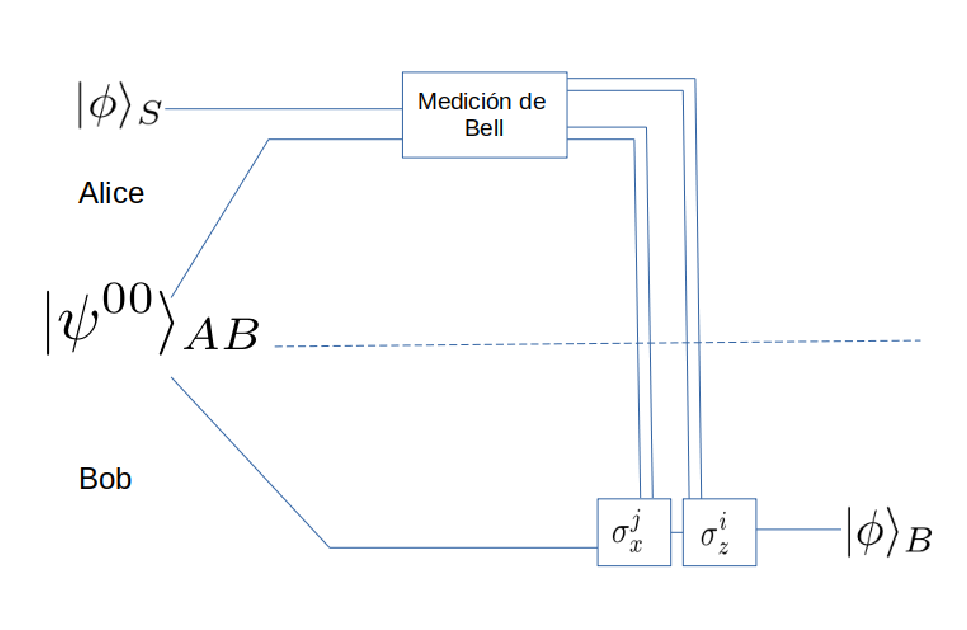
\includegraphics[scale=0.20]{./teletransportation_protocol.png}
\end{center}
\caption{Quantum teleportation protocol.}
\label{fig::qt_protocol}
\end{figure}\\
\linebreak
\pagebreak
\newpage
The steps of the protocol are the following:
\begin{enumerate}
\item Alice measures the system $SA$ in the Bell basis. To see how this works, consider the following table:
\begin{center}
\begin{tabular}{ |c|c| }
 \hline
 Alice Measures & Bob's State\\ \hline
 $|\psi^{00}\rangle$  & $|\phi\rangle_B$\\\hline
 $|\psi^{01}\rangle$  & $\sigma_x|\phi\rangle_B$\\\hline
 $|\psi^{10}\rangle$  & $\sigma_z|\phi\rangle_B$\\\hline
 $|\psi^{11}\rangle$  & $\sigma_x\sigma_z|\phi\rangle_B$\\
 \hline
\end{tabular}
\end{center}

\item Alice sends the result of the Bell measurement to Bob; that is, she sends two classical bits $i,j \in \{0,1\}$.
\item Bob applies $\sigma_z^i\sigma_x^j$ to his state and obtains $|\phi\rangle_B$.
\end{enumerate}
It is important to note that when Alice performed the Bell measurement, her state collapsed. Therefore, she no longer has the initial state $|\phi\rangle$. This is expected because of the no-cloning theorem of quantum mechanics: Alice cannot copy her state; she can only send it to Bob, destroying her own state in the process.

\begin{thebibliography}{99}
%% The bibliography is ordered alphabetically by the surname of the author or main author.
%% Each entry has its own formatting depending on whether it is a book, article,
%% thesis, web resource, etc.

\bibitem{Bell} J.S. Bell. \textit{On the Einstein Podolski Rosen Paradox}. \url{https://cds.cern.ch/record/111654/files/vol1p195-200_001.pdf}

\bibitem{Nielsen} Michael A. Nielsen, Isaac L. Chuang. \textit{Quantum Computation and Quantum Information}. Cambridge University Press 2010. 10th Anniversary Edition.

\bibitem{Feynman} Richard P. Feynman. \textit{Simulating Physics with Computers.} \url{https://doi.org/10.1007/BF02650179}.

\bibitem{Qiskit} \textit{Qiskit Textbook}. \url{https://qiskit.org/textbook-beta}

\bibitem{Mermin} N. David Mermin. \textit{Quantum Computer Science: An Introduction}. Cambridge University Press, 2007.

\bibitem{Sakurai} J.J. Sakurai. \textit{Modern Quantum Mechanics}. The Benjamin/Cummings Publishing Company, 1985.

\bibitem{Dotsenko} Viktor Dotsenko. \textit{An Introduction to the Theory of Spin Glasses and Neural Networks}. World Scientific 1994.

\bibitem{Bahri} Yasaman Bahri, Jonathan Kadmon, Jeffrey Pennington, Sam S. Schoenholz, Jascha Sohl-Dickstein, Surya Ganguli. \textit{Statistical Mechanics of Deep Learning}. \url{https://www.annualreviews.org/doi/pdf/10.1146/annurev-conmatphys-031119-050745}

%\bibitem{Hopfield} J.J. Hopfield. \textit{Neural Networks and physical systems with emergent collective computational abilities}. \url{https://doi.org/10.1073/pnas.79.8.2554}

%\bibitem{McCulloch} Warren S. McChulloch, Walter H. Pitts. \textit{A LOGICAL CALCULUS OF THE IDEAS IMMANENT IN NERVOUS ACTIVITY}. \url{http://www.cse.chalmers.se/~coquand/AUTOMATA/mcp.pdf}

\end{thebibliography}
\end{document}
